\documentclass[journal,12pt,twocolumn]{IEEEtran}
\usepackage{amsthm}
\usepackage{graphicx}
\usepackage{mathrsfs}
\usepackage{txfonts}
\usepackage{stfloats}
\usepackage{pgfplots}
\usepackage{cite}
\usepackage{cases}
\usepackage{mathtools}
\usepackage{caption}
\usepackage{enumerate}	
\usepackage{enumitem}
\usepackage{amsmath}
\usepackage[utf8]{inputenc}
\usepackage[english]{babel}
\usepackage{multicol}
%\usepackage{xtab}
\usepackage{longtable}
\usepackage{multirow}
%\usepackage{algorithm}
%\usepackage{algpseudocode}
\usepackage{enumitem}
\usepackage{mathtools}
\usepackage{gensymb}
\usepackage{hyperref}
%\usepackage[framemethod=tikz]{mdframed}
\usepackage{listings}
    %\usepackage[latin1]{inputenc}                                 %%
    \usepackage{color}                                            %%
    \usepackage{array}                                            %%
    \usepackage{longtable}                                        %%
    \usepackage{calc}                                             %%
    \usepackage{multirow}                                         %%
    \usepackage{hhline}                                           %%
    \usepackage{ifthen}                                         %%
  \providecommand{\nCr}[2]{\,^{#1}C_{#2}}
  \providecommand{\nPr}[2]{\,^{#1}P_{#2}}
  \lstset{
%language=C,
frame=single, 
breaklines=true,
columns=fullflexible
}

\title{Compulsory Assignment
\\Probability and Random Variables }
\author{Swati Mohanty (EE20RESCH11007) }
\date{April 2021}

\begin{document}

\maketitle

\section{Problem}
Let, $X_1 \sim Bin(n_1, p)$ and $X_2 \sim Bin(n_2, q)$, independently. Find the PMF of $X_1 - X_2.$
\section{Solution}
Given, $X_1 \sim Bin(n_1, p)$ and $X_2 \sim Bin(n_2, q)$, independently.\\
$\therefore n_2-X_2 \sim Bin(n_2, p)$\\
By additive/ reproductive property of binomial,\\
$X_1+n_2-X_2 \sim Bin(n_1+n_2, p)$\\
Let, $D= X_1 -X_2$.
\begin{align}
    P(D=d) &= P(X_1 -X_2 = d)\\
    &= P(X_1 -X_2 +n_2 = d +n_2)\\
    &= \binom{n_1+n_2}{n_2+d} p^{n_2+d} q^{n_1-d}, d= -n_2\ \text{to}\ n_1\ \label{subtraction}
\end{align}
\begin{figure}[!ht]
\centering
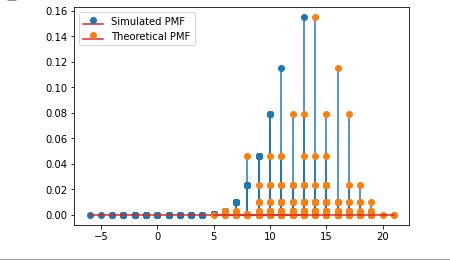
\includegraphics[width=\columnwidth]{comp pmf.PNG}
\caption{Probability Mass Function}
\label{fig:pmf}
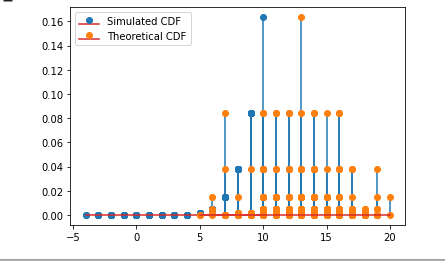
\includegraphics[width=\columnwidth]{comp cdf.PNG}
\caption{CDF}
\label{fig:cdf}
\end{figure}
\section{Problem}
Let X represent the difference between the
number of heads and the number of tails
obtained when a coin is tossed 6 times. What
are possible values of X?
\section{Solution}
Q3.7)Let $X_1$ denotes the number of heads and $X_2$ denotes the number of tails that occur when a coin is tossed 6 times.\\
We get, $X_1 \sim Bin(n=6, p)$\\
and $X_2 \sim Bin(n=6,1-p=q)$.\\
$\therefore n-X_2 \sim Bin(6, p)$.\\
By reproductive property,
\begin{align}
    X_1+n-X_2 \sim Bin(6+6, p)
\end{align}

$X=X_1-X_2$. Using \eqref{subtraction},
\begin{align}
    P(X=x) = \binom{6+6}{6+x} p^{6+x} q^{6-x}, x= -6\ \text{to}\ 6 
\end{align}
Suppose, the coin is unbiased. Then, $p=q= \frac{1}{2}$.
\begin{align}
    \therefore P(X=x) = \binom{12}{6+x}\brak{\frac{1}{2}}^{12}, x= -6\ \text{to}\ 6 
\end{align}

\textbf{Download python code from here}\\
\begin{lstlisting}
https://github.com/Swati-Mohanty/AI5002/blob/main/Compulsory Assignment/codes/comp.py
\end{lstlisting}
\textbf{Download latex code from here-}\\
\begin{lstlisting}
https://github.com/Swati-Mohanty/AI5002/blob/main/Compulsory Assignment/codes/compulsory.tex
\end{lstlisting}
\end{document}
